% !TEX root = ../main.tex
\section{Q12: Vertikal integrasjon vs.\ outsourcing -- hold-up, free-rider, double markup}\label{q:12}

\begin{quote}
\emph{Præsenter begreberne vertikal integration og outsourcing / market transactions og redegør for principielle fordele og ulemper ved de respektive organiseringsalternativer. Diskuter i denne forbindelse kontraktmæssige aspekter af interaktion mellem virksomheden og dens leverandører/distributører -- herunder: hold-up problemer, free-rider problemer, double markup problemer.}
\end{quote}

\subsection*{Svar (kort)}
Vertikal integrasjon og outsourcing er to ytterpunkter på et organiseringskontinuum; fordeler og ulemper følger av \thref{costly-contracting}{costly contracting} og informasjonsasymmetri. De tre kontraktproblemene -- hold-up, free-rider og double markup -- er distinkte årsaker til at markedskontrakter mellom uavhengige parter feiler, og hver peker mot vertikal integrasjon (eller spesifikke kontraktsdesign) som løsning. Hold-up skyldes relasjonsspesifikke investeringer, free-riding skyldes positive eksternaliteter mellom distributører, og double markup skyldes uavhengig prissetting av to suksessive monopolister. [SLIDE]

\subsection*{Relevante teorier (kort)}

\paragraph{\thref{vertical-integration-outsourcing}{Vertikal integrasjon og outsourcing (bredt)}\quad\SOne/\SThree}
Outsourcing gir markedsdisiplin, skalafordeler, fleksibilitet og sterkere insentiver. Integrasjon gir kontroll, koordinasjon, IP-beskyttelse og eliminering av kontraktproblemer. Valget er en trade-off mellom transaksjonskostnader i markedet og \thref{agency-costs}{agency costs} internt. Se Q11 for koblingen til Boundaries of the Firm, eierskap og market power. [SLIDE]

\paragraph{\thref{hold-up-problem}{Hold-up-problemet}\quad\SOne/\SThree}
Når en part investerer i \emph{relasjonsspesifikke aktiva} -- altså investeringer som er mye mer verdt i akkurat denne relasjonen enn andre steder (lav alternativverdi) -- kan motparten i ettertid (\emph{ex post}) reforhandle og kapre \emph{quasi-renter}: differansen $V - V_0$ mellom verdien i relasjonen ($V$) og verdien i nest-beste anvendelse ($V_0$). Konsekvens: rasjonelle parter forutser dette og underinvesterer i forkant (\emph{ex ante}). Løsninger: vertikal integrasjon (samme eier eliminerer reforhandling), langsiktige kontrakter, gjensidig avhengighet (hver part har egne spesifikke aktiva som ``gissel''), og reputasjon. Klassisk eksempel: GM--Fisher Body på 1920-tallet. Williamsons fem typer asset specificity (site -- lokasjon; physical -- spesialisert utstyr; human -- spesialisert kompetanse; dedicated -- kapasitet bygget kun for én kunde; temporal -- tidssensitivitet) bestemmer hold-up-risikoen. [SLIDE/BOK]

\paragraph{\thref{free-rider-problem}{Free-rider-problemet (nedstrøms)}\quad\SThree}
Uavhengige distributører underinvesterer i service og markedsføring fordi gevinsten fanges av konkurrerende forhandlere (\emph{inter-dealer free-riding}). Klassisk eksempel: kunden bruker high-service-forhandleren (stort showroom, god rådgivning) til å bestemme seg, og kjøper deretter billigere hos en discount-forhandler som ikke har slike kostnader. Dette kalles \emph{showrooming}: kunden ``viser fram'' produktet i én butikk, kjøper i en annen. Resultat: ingen vil bygge showroomet -- service-nivået kollapser. Løsninger: vertikal integrasjon (produsenten eier distribusjonen selv), franchise med servicekrav, eksklusive territorier (én forhandler per geografisk område), og \emph{RPM} (\emph{Resale Price Maintenance} -- produsenten setter en minste videresalgspris og forbyr priskonkurranse nedstrøms, slik at margingrunnlaget for å yte service bevares). [BOK]

\begin{tcolorbox}[colback=blue!4, colframe=blue!50!black, boxrule=0.4pt, arc=2pt, left=6pt, right=6pt, top=4pt, bottom=4pt]
\textbf{Intuisjon:} Free-rider = du høster gevinsten av andres investering uten å bidra. McDonald's-franchisee på Gardermoen investerer ikke i kvalitet -- eksternalitet = påfører andre kostnad; free-rider = tar andres gevinst. Begge gir underinvestering -- ulik mekanisme.
\end{tcolorbox}

\paragraph{\thref{double-markup-problem}{Double markup-problemet}\quad\SOne}
To suksessive monopolister i samme verdikjede setter prisen uavhengig av hverandre, og hver legger på sin egen markup (påslag). Resultat: \emph{dobbelt} markup -- oppstrøms margin pluss nedstrøms margin -- gir sluttforbrukerpris høyere og kvantum lavere enn det som er optimalt for verdikjeden samlet. Talleksempel: marginalkostnad $c=20$, oppstrømsprisen $P_w=60$ (45 \% markup), sluttpris $P_{\text{slutt}}=80$, kvantum $Q=20$. Hvis de to integrerer (én aktør, én markup): $P=60$, $Q=40$ -- +33\% profitt og +100\% kvantum. Kontraktuelle alternativer som unngår full integrasjon: \emph{two-part tariff} (en fast avgift pluss enhetspris -- f.eks.\ engangsgebyr + lav pris per enhet), \emph{franchise fee} (engangsbeløp for retten til å selge), eller RPM (Resale Price Maintenance -- produsenten setter videresalgsprisen direkte). Forutsetter monopol i begge ledd; med konkurranse nedstrøms forsvinner $D$s markup uansett. [SLIDE]

\subsection*{Illustrasjoner fra forelesning}

\begin{figure}[H]
  \centering
  
\includegraphics[width=0.55\linewidth]{BSZ_kap_10_2026/by_slide/slide_017/BSZ_kap_10_2026_slide_017_asset_01_image7.jpeg}
  \caption{Tautrekking mellom parter -- illustrerer hold-up-problemet: når begge parter har investert, oppstår forhandlingskonflikt om quasi-renter. (BSZ kap.\ 10, slide 17) [SLIDE]}
\end{figure}

\begin{figure}[H]
  \centering
  
\includegraphics[width=0.45\linewidth]{BSZ_kap_9_2026/by_slide/slide_015/BSZ_kap_9_2026_slide_015_asset_01_image4.jpeg}
  \caption{Oppvasken ingen tar -- illustrerer free-rider-problemet: alle nyter godt av at jobben gjøres, men ingen vil bære kostnaden. (BSZ kap.\ 9, slide 15) [SLIDE]}
\end{figure}

\subsection*{Illustrasjon -- de tre kontraktproblemene}

\begin{center}
\renewcommand{\arraystretch}{1.2}
\begin{tabular}{@{}p{2.8cm}p{3.5cm}p{3.5cm}p{3.5cm}@{}}
\toprule
 & \textbf{Hold-up} & \textbf{Free-rider} & \textbf{Double markup} \\
\midrule
\textbf{Kilde} & Spesifikke investeringer & Positiv eksternalitet mellom dist. & Suksessive monopolister \\
\textbf{Mekanisme} & Reforhandling ex post & Underinvestering i service & Dobbel prispåslag \\
\textbf{Konsekvens} & Underinvestering ex ante & Merkevare eroderes & For høy pris, for lavt $Q$ \\
\textbf{VI-løsning} & Felles eierskap & Eie distribusjon & Fjerne én markup \\
\textbf{Kontraktsløsning} & Langsiktig k., penalty & Franchise, eksklusive terr. & Two-part tariff, RPM \\
\bottomrule
\end{tabular}
\end{center}
\textit{Tabell: Sammenligning av de tre kontraktproblemene og deres løsninger. [SLIDE/BOK]}

\subsection*{Illustrasjon -- double markup (grafisk)}

\begin{figure}[H]
\centering
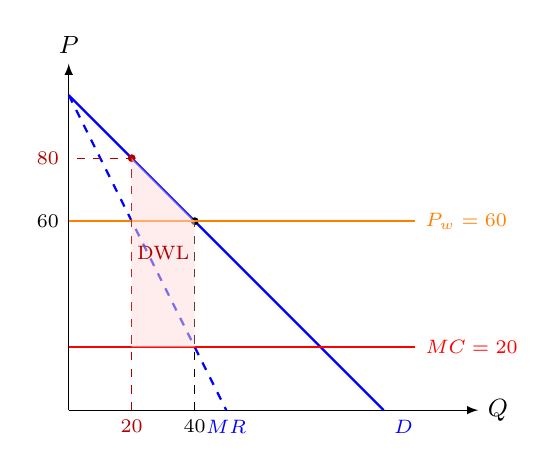
\begin{tikzpicture}[>=latex, scale=0.8, every node/.style={font=\small}]
  \draw[->] (0,0) -- (6.5,0) node[right] {$Q$};
  \draw[->] (0,0) -- (0,5.5) node[above] {$P$};
  \draw[thick, blue] (0,5) -- (5,0) node[below right] {\scriptsize $D$};
  \draw[thick, blue, dashed] (0,5) -- (2.5,0) node[below] {\scriptsize $MR$};
  \draw[thick, red] (0,1.0) -- (5.5,1.0) node[right] {\scriptsize $MC=20$};
  % Integrert
  \filldraw[black] (2.0,3.0) circle (1.5pt);
  \draw[dashed] (2.0,0) -- (2.0,3.0) -- (0,3.0);
  \node[below] at (2.0,0) {\scriptsize $40$};
  \node[left] at (0,3.0) {\scriptsize $60$};
  % Double markup
  \draw[thick, orange] (0,3.0) -- (5.5,3.0) node[right] {\scriptsize $P_w=60$};
  \filldraw[red!70!black] (1.0,4.0) circle (1.5pt);
  \draw[dashed, red!70!black] (1.0,0) -- (1.0,4.0) -- (0,4.0);
  \node[below, red!70!black] at (1.0,0) {\scriptsize $20$};
  \node[left, red!70!black] at (0,4.0) {\scriptsize $80$};
  % DWL
  \fill[red!15, opacity=0.5] (1.0,4.0) -- (2.0,3.0) -- (2.0,1.0) -- (1.0,1.0) -- cycle;
  \node[font=\scriptsize, red!70!black] at (1.5,2.5) {DWL};
\end{tikzpicture}
\caption{Double markup: uintegrert $P=80, Q=20$ (rødt) vs.\ integrert $P=60, Q=40$ (svart). [BOK]}
\end{figure}

\subsection*{Real-world eksempler}

\textbf{Eks.~1 -- IKEA og leverandørrelasjoner (hold-up og kontraktsdesign).}\quad [EKS]
IKEA designer produkter som krever \emph{dedikerte} produksjonslinjer hos leverandører i Øst-Europa og Asia (physical + dedicated asset specificity). For å unngå hold-up bruker IKEA flerårige rammeavtaler med volum-garantier, kvalitetsinspeksjoner (monitoring) og gradvis diversifisering av leverandørbasen. IKEA integrerer \emph{ikke} vertikalt i produksjon -- kontraktsløsningen er billigere enn integrasjon fordi produktene er modulære (moderat spesifisitet).

\textbf{Eks.~2 -- McDonald's (free-rider og franchising), sammenligning.}\quad [EKS]
McDonald's løser free-rider-problemet gjennom \emph{franchising} med strenge servicekrav: kvalitetsstandarder, renhold, menyer og opplæring kontrolleres sentralt. Franchisetaker som leverer dårlig kvalitet skader merket (free-riding) og mister lisensen. Kontrast med IKEA: McDonald's nedstrømsproblem (distributør free-rider) løses med franchise, mens IKEAs oppstrømsproblem (leverandør hold-up) løses med rammeavtaler. Begge unngår full integrasjon fordi kontraktsdesign er tilstrekkelig -- men forutsetter effektiv monitoring.

\subsection*{Kobling til Mærsk Power-to-X}
PtX-verdikjeden illustrerer alle tre kontraktproblemene: [CASE]
\begin{itemize}\setlength{\itemsep}{2pt}
\item \textbf{Hold-up:} Elektrolyseanlegg bygget til Mærsks spesifikasjon er et spesifikt aktivum. Leverandøren (f.eks.\ Siemens Energy) kan holdes opp etter investering -- Mærsks løsning: milestone-betalinger, performance guarantees, step-in-rettigheter.
\item \textbf{Free-rider:} Mærsk samarbeider med andre rederier i bransjeinitiativ for grønt drivstoff. Uten forpliktende kontrakter kan partnere free-ride på Mærsks investeringer i infrastruktur.
\item \textbf{Double markup:} Hvis elektrolyseprodusent og e-metanol-produsent begge har markedsmakt, kan dobbel markup drive opp drivstoffprisen. Mærsks interesse i bakoverintegrasjon til elektrolyse eliminerer dette leddet.
\end{itemize}

\subsection*{Fallgruber}
\begin{itemize}\setlength{\itemsep}{2pt}
\item Forveksle Q12 med Q11: Q12 handler om \emph{kontraktproblemer}; Q11 handler om \emph{Boundaries of the Firm} og \emph{market power}.
\item Kun beskrive VI-fordeler uten å nevne kontraktsalternativer (franchise, two-part tariff, RPM).
\item Forveksle hold-up (ex post reforhandling) med moral hazard (skjult handling) -- overlappende men distinkte.
\item Glemme double markup-tallet: vis det numeriske eksemplet ($Q: 20\to 40$, $\pi: 1200\to 1600$).
\item Ikke nevne asset specificity-typene ved hold-up -- Williamson krever det.
\item Behandle free-rider som generelt kollektiv handlingsproblem -- i VI-konteksten er det spesifikt om distributører.
\end{itemize}

\FloatBarrier
\subsection*{Håndskrivbar disposisjon (15-min forberedelse)}
\begin{itemize}\setlength{\itemsep}{2pt}
\item \textbf{Tese:} Tre kontraktproblemer (hold-up, free-rider, double markup) forklarer når outsourcing feiler og VI lønner seg.
\item \thref{vertical-integration-outsourcing}{VI vs.\ outsourcing}: fordeler/ulemper kort (markedsdisiplin vs.\ kontroll).
\item \textbf{Hold-up:} spesifikke aktiva $\Rightarrow$ quasi-rente approprieres $\Rightarrow$ underinvestering. 5 typer asset specificity. Løsning: VI, langsiktig kontrakt, mutual hostage.
\item \textbf{Free-rider:} distributør underinvesterer i service. Showrooming. Løsning: franchise, eksklusive terr., RPM.
\item \textbf{Double markup:} $c=20, P_w=60, P=80, Q=20$ vs.\ integrert $P=60, Q=40$. Løsning: VI, two-part tariff.
\item Tabell: sammenligning av de tre problemene (kilde, mekanisme, løsning).
\item Eks.\ 1: IKEA (hold-up, rammeavtaler). Eks.\ 2: McDonald's (free-rider, franchise).
\item Case: Mærsk PtX -- alle tre problemene representert.
\item Søyle: \SOne\ (eierskap/kontroll) + \SThree\ (insentivdesign for leverandører/distributører).
\end{itemize}
